% ==============================================================================
% PAGE 18: 3) COLD WATER STORAGE TANK (Pre-Heating Unit) (Numbered Page 10)
% ==============================================================================
\subsubsection*{3) COLD WATER STORAGE TANK (Pre-Heating Unit)}

\begin{center}
  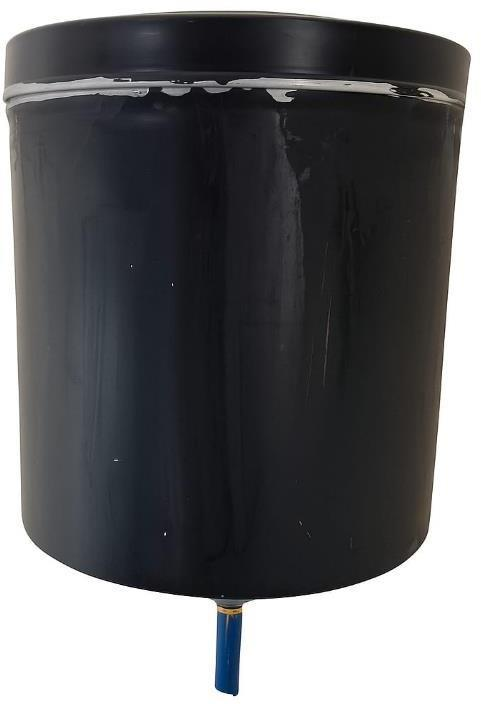
\includegraphics[width=50mm]{figures/fig3_cold_water_storage_tank.jpg}
\end{center}

\noindent
\begin{spacing}{1.2}
{\fontsize{10.2}{14.5}\selectfont
A black-colored cold storage water tank is installed as a pre-heating unit in the system. It serves two purposes:\\[3mm]
\textbf{SPECIFICATION:}
\begin{enumerate}[leftmargin=8mm, itemsep=2mm]
  \item \textbf{Pre-heating of water:} The black surface absorbs solar radiation effectively, slightly increasing the temperature of the water before it enters the copper receiver. This pre-heating process improves overall system efficiency and reduces the time required to reach the desired hot-water temperature.
  \item \textbf{Storage:} The tank also acts as a temporary storage reservoir that supplies a steady flow of water to the parabolic collector.\\[1.5mm]
  The tank is made of lightweight aluminium material, coated with black paint to maximize solar absorption.\\[1.5mm]
  A small outlet at the bottom connects to the copper receiver tube through a flexible pipe. This simple addition improves energy utilization and makes the design cost-effective and efficient.
  \item \textbf{Capacity of the tank :} 5 lit
\end{enumerate}
}
\end{spacing}
\clearpage
